\chapter{System Architecture \& Lifecycle Phases}
\label{chap:system_architecture}

This chapter details the unified 4-phase architecture of the autonomous PDDL lifecycle agent. The framework is structured into four closed-loop modules aligned with the KEPS Software Development Life Cycle (\gls{sdlc}).

\section{Architectural Overview}
Figure~\ref{fig:block_diagram_placeholder} provides a high-level overview of the closed-loop agent workflow. The architecture operates across four specialized containers:
\begin{enumerate}
    \item \textbf{Phase 1 (Blue): Knowledge Ingestion \& AST Extraction}
    \item \textbf{Phase 2 (Green): Formulation, AST Schema Enforcer \& Deterministic Compiler}
    \item \textbf{Phase 3 (Orange): Verification, Symbolic Oracles, Layered Triage \& Targeted AST Repair}
    \item \textbf{Phase 4 (Grey): Maintenance, Evolution \& Regression Evaluation Suite}
\end{enumerate}

\begin{figure}[htbp]
\centering
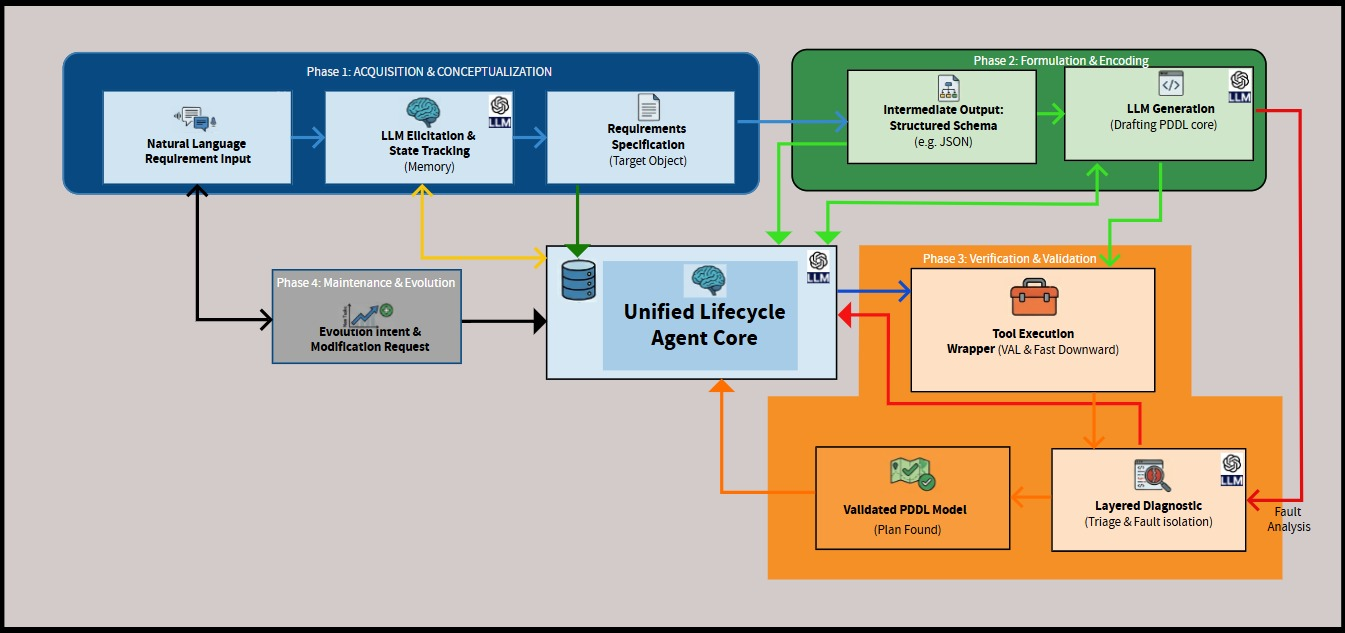
\includegraphics[width=0.95\textwidth]{figures/Block_diagram.jpeg}
\caption{Unified 4-Phase Closed-Loop PDDL Lifecycle Agent Architecture.}
\label{fig:block_diagram_placeholder}
\end{figure}

\section{Phase 1: Knowledge Ingestion \& AST Extraction}
Phase 1 accepts raw, unconstrained natural language requirement descriptions $R_{\text{nl}}$ and extracts grounded structural components into an initial JSON object blueprint $B_0$.

\subsection{Ingestion Contracts}
The ingestion engine extracts three core conceptual elements:
\begin{itemize}
    \item \textbf{Type Hierarchy:} Mappings of parent-child single inheritance relations (e.g., \texttt{truck - location}).
    \item \textbf{Predicate Signatures:} Parameter lists and variable bindings defining environmental facts.
    \item \textbf{Action Schemas:} Parameter signatures, preconditions, and add/delete state transition effects.
\end{itemize}

\section{Phase 2: Formulation \& Encoding (Deterministic Compiler)}
Phase 2 converts conceptual objects into syntactically valid PDDL files without relying on the LLM to generate raw Lisp strings.

\subsection{Intermediate AST Contract: \texttt{DomainBlueprint}}
To prevent syntax collapse, Phase 2 enforces a strict Pydantic JSON Abstract Syntax Tree (\gls{ast}) schema (\texttt{DomainBlueprint}). By forcing the LLM to output structured JSON rather than S-expressions, language understanding is completely decoupled from PDDL syntax formatting.

\subsection{Deterministic Programmatic Lisp Compiler}
The generation module passes the validated \texttt{DomainBlueprint} to a deterministic programmatic compiler (\texttt{compile\_pddl\_programmatically}), which constructs the target PDDL text:
\begin{enumerate}[label=(\alph*)]
    \item \textbf{Type Normalization:} Formats single-type hierarchy blocks and eliminates circular inheritance.
    \item \textbf{Predicate Compilation:} Auto-injects variable tags (\texttt{?x}) and parameter type signatures.
    \item \textbf{Action S-Expression Construction:} Programmatically constructs \texttt{:action}, \texttt{:parameters}, \texttt{:precondition}, and \texttt{:effect} blocks with guaranteed parenthesis balance:
    \begin{lstlisting}[language=pddl, caption=Compiled PDDL Action Schema Example]
(:action drive
  :parameters (?v - truck ?from - location ?to - location)
  :precondition (and (at ?v ?from) (connected ?from ?to))
  :effect (and (not (at ?v ?from)) (at ?v ?to)))
    \end{lstlisting}
\end{enumerate}
Phase 2 achieves a \textbf{100\% Syntax Validity Rate}, completely eliminating unmatched parentheses and colon keyword hallucinations.

\section{Phase 3: Verification, Layered Triage \& Targeted Repair}
Phase 3 establishes a multi-tier closed-loop verification and model repair pipeline.

\subsection{Symbolic Tool Oracles (VAL \& Fast Downward)}
The Validation Node executes binary symbolic tools on compiled PDDL domain and problem pairs ($S_{\text{pddl}}, P_{\text{pddl}}$):
\begin{itemize}
    \item \textbf{VAL Validator Oracle}~\cite{howey2004}: Evaluates static PDDL syntax, parameter type consistency, and plan execution state transitions $S_{i+1} = (S_i \setminus \text{eff}^-(a_i)) \cup \text{eff}^+(a_i)$.
    \item \textbf{Fast Downward Planner Oracle}~\cite{helmert2006}: Translates PDDL into SAS+ representations, constructs causal graphs, and executes $A^*$ search to verify plan solvability.
\end{itemize}

\subsection{Layered Diagnostic Triage}
If an Oracle returns a failure signal, the Layered Diagnostic Engine (\texttt{nodes/triage.py}) categorizes the failure mode:
\begin{equation}
\text{Failure Category} \in \{\text{SYNTAX\_ERROR}, \text{TYPE\_MISMATCH}, \text{GROUNDING\_UNSOLVABLE}\}
\end{equation}

\subsection{Spectrum-Based Fault Suspiciousness Scoring \texorpdfstring{$\sigma(n)$}{sigma(n)}}
To prevent unconstrained global re-prompting, the diagnostic engine calculates a fault suspiciousness rank score $\sigma(n) \in [0.0, 1.0]$ across all AST action nodes $n \in B_{\text{domain}}$:
\begin{equation}
\sigma(n) = \frac{e_{\text{fail}}(n)}{\sqrt{e_{\text{total}}(n) \cdot e_{\text{fail\_total}}}}
\end{equation}
where $e_{\text{fail}}(n)$ denotes execution trace errors associated with action node $n$.

\subsection{Targeted AST Repair \& Feedback Loop}
The Repair Node (\texttt{nodes/repair.py}) isolates the sub-schema associated with the highest suspiciousness score $\sigma(n)$ (e.g., a specific action precondition list) and prompts the LLM to patch only that isolated node. The modified AST is re-compiled in Phase 2 and re-validated in Phase 3, forming a closed feedback loop that converges in an average of \textbf{1.2 iterations}.

\section{Phase 4: Maintenance, Evolution \& Regression Testing}
Phase 4 manages continuous domain evolution through the Evolution Manager (\texttt{nodes/maintenance.py}). When new domain requirements or modified actions are introduced, Phase 4 re-routes modification requests back to Phase 1. 

To prevent semantic regressions, Phase 4 evaluates modified domains against a historical regression suite $\mathcal{K}_{\text{maint}} = \{P_1, P_2, \dots, P_k\}$ of problem instances, ensuring backward compatibility across evolving domain models.
